\section{Die Normalform}
    \begin{theorem}[Existenz einer Normalform]\label{thm:normal_form}
        Jeder einfach zusammenh\"angende \((n\geq6)\)-dimensionalen H-Kobordismus besitzt f\"ur jedes \(2\leq k\leq n-3\) eine Henkelzerlegung, die lediglich \(k\)- und \((k+1)\)-Henkel besitzt. 
    \end{theorem}
    \begin{proof}
        Es wird \"uber Induktion nach \(k\) gezeigt, dass eine Darstellung ohne \(j\)-Henkel f\"ur \(j<k\) existiert, also dass \(\mathcal{W}_{k-1}\cong\mathcal{M}\times\mathbb{I}\) gilt. Der Induktionsanfang \(k=2\) ist gerade die Aussage von Satz \ref{thm:one_handle_rem}.
            
        \subsubsection*{Induktionsschritt}
            Sei die Aussage f\"ur \(k\) bereits gezeigt, dann existiert eine Henkelzerlegung von \(\mathcal{W}\) mit \(\mathcal{W}_{k-1}=\mathcal{M}\times\mathbb{I}\) und f\"ur das Differential in den Homologiegruppen gilt \(\dx_{k+1}=\partial_{k+1}\). Dieses ist wegen der langen exakten Folge
            \begin{center}
                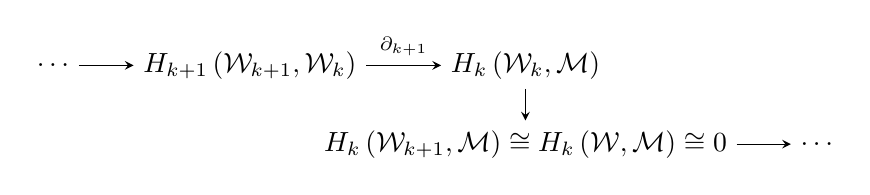
\begin{tikzpicture}
                    \path   node (A) at (-6, 1) {\(\dots\)}
                            node (B) at (-3.5, 1) {\(H_{k+1}\left(\mathcal{W}_{k+1},\mathcal{W}_k\right)\)}
                            node (C) at (0, 1) {\(H_k\left(\mathcal{W}_k,\mathcal{M}\right)\)}
                            node (D) at (0, 0) {\(H_k\left(\mathcal{W}_{k+1},\mathcal{M}\right)\cong H_k\left(\mathcal{W},\mathcal{M}\right)\cong0\)}
                            node (E) at (3.7, 0) {\(\dots\)};
                    \draw[-stealth] (A.east) -- (B.west);
                    \draw[-stealth] (B.east) -- node[above, pos = 0.5] {\scriptsize\(\partial_{k+1}\)} (C.west);
                    \draw[-stealth] (C.south) -- (D.north);
                    \draw[-stealth] (D.east) -- (E.west);
                \end{tikzpicture}
            \end{center}
            ein Epimorphismus. Somit existiert f\"ur alle \(\Psi^k\in H_k\left(\mathcal{W}_k,\mathcal{M}\right)\) ein Element 
            \[\sum_{j=1}^{c_{k+1}}x_j\Psi_j^{k+1}\in H_{k+1}\left(\mathcal{W}_{k+1},\mathcal{W}_k\right),\,\quad\text{sodass}\quad\sum_{j=1}^{c_{k+1}}x_j\dx\Psi_j^{k+1}=\Psi^k\quad\text{gilt.}\]
            Sei \(\Phi^{k+1}\) ein trivialer Henkel, ist die Anklebesph\"are kontrahierbar, und somit \(\dx\Phi^{k+1}=0\). Folglich existiert gem\"a\ss{} dem Modifikationssatz \ref{prop:modification} ein zu \(\Phi^{k+1}\) isotoper Henkel \(\chi^{k+1}\) mit
            \[\dx\chi^{k+1}=\dx\Phi^{k+1}+\sum_{j=1}^{c_{k+1}}x_j\dx\Psi_j^{k+1}=0+\Psi^k=\Psi^k\,.\]
            Gem\"a\ss{} dem Homologie-Lemma \ref{thm:homology} existiert ein zu \(\chi^{k+1}\) isotoper Henkel, der den G\"urtel von \(\Psi^k\) transversal und in genau einem Punkt schneide, sodass Korollar \ref{cor:handle_replacement} die Ersetzung von \(\Psi^k\) mit einem \((k+2)\)-Henkel erm\"oglicht. 
            
            Durch \"Ubergang zu der dualen Repr\"asentation k\"onnen \(j\)-Henkel f\"ur \(j>k+1\) in \((n-j)\)-Henkel \"uberf\"uhrt werden und eine Anwendung der oberen Induktion mit \(k^{\prime}=n-k\) zeigt die Aussage.
    \end{proof}
    
\section{Differentialmatrizen}
    Sei \(H^k\left(\mathcal{W}_k,\mathcal{W}_{k-1}\right)\cong\mathbb{Z}^{c_k}\) als \(\mathbb{Z}\)-Modul mit der kanonischen Basis aufgefasst, kann die Abbildungsmatrix \(M_k\in\mathbb{Z}^{c_k\times c_{k-1}}\) des Differentials \(\dx_k\) definiert werden. Diese ist stets von der gegebenen Henkelzerlegung abh\"angig. Aus der Existenz einer Normalform folgt, dass lediglich ein \(k\) betrachtet werden muss. Elementare Zeilenoperationen auf dieser Matrix ergeben nun Matrizen, die mit weiteren Henkelzerlegungen von \(\mathcal{W}\) korrespondieren. Somit kann ein H-Kobordismus und das Entfernen oder Hinzuf\"ugen von Henkeln durch wenige Daten beschrieben, und mithilfe des Gau\ss schen Eliminationsverfahrens deutlich vereinfacht werden. 
    
    \subsection{Elementare Zeilenoperationen}
        Dass eine Zeile zu einer andere Zeile addiert werden kann folgt aus dem Modifikationslemma. Ist die Matrix von der Form 
        \[A=\begin{pmatrix}
            B & 0\\
            0 & 1
        \end{pmatrix}\,,\]
        ergibt das Homologie-Lemma \ref{thm:homology} eine Henkelzerlegung mit Differentialmatrix \(B\). Zeilenvertauschungen korrespondieren mit einer Umnummerierung der Henkel und eine Skalierung einer Zeile mit \(-1\) ist \"aquivalent mit der Umorientierung des zugeh\"origen Kerns.
        
    \begin{theorem}[H-Kobordismus-Satz]
        Jeder mindestens \(6\)-dimensionale, einfach zusammenh\"angende H-Ko\-bor\-dis\-mus \((\mathcal{W},\mathcal{M},-)\) ist trivial.
    \end{theorem}
    \begin{proof}
        Anwenden des gau\ss schen Eliminationsverfahrens auf die Differentialmatrix einer Normalform ergibt eine Henkelzerlegung, deren Differentialmatrix die Identit\"at ist. Wiederholte Reduktion dieser resultiert in der leeren Matrix, die eine Henkelzerlegung ohne Henkel repr\"asentiert. Es folgt 
        \[\mathcal{W}\cong\mathcal{W}_n\cong\mathcal{W}_{-1}=\mathcal{M}\times\mathbb{I}\,.\]
    \end{proof}